\documentclass[
size=17pt,
paper=smartboard,
mode=present,
display=slidesnotes,
style=paintings,
nopagebreaks,
blackslide,
fleqn]{powerdot}

% styles: sailor, paintings
% wj capsules prettybox
% mode = handout or present


\newcommand{\palette}{Moitessier}
% palettes:
%    - sailor: Sea, River, Wine, Chocolate, Cocktail 
%    - paintings: Syndics, Skater, GoldenGate, Moitessier, PearlEarring, Lamentation, HolyWood, Europa, MayThird, Charon 

\newcommand{\cursopequeno}{EC01045 PDS}
\newcommand{\cursogrande}{\Large EC01045 -- Processamento digital de sinais}

\usepackage{amsmath,graphicx,color,amsfonts}
\usepackage[brazilian]{babel}
\usepackage[utf8]{inputenc}
\usepackage{bbding}

\author{Ronaldo de Freitas Zampolo\\FCT-ITEC-UFPA}
\date{ERE 2020}


\pdsetup{
   lf = {\cursopequeno},
   rf = {Transformada Z},
   palette = \palette,randomdots={false},
   cf={\theslide}
}

\title{\cursogrande\\ \vspace{1cm}Transformada Z}

\begin{document}
   \maketitle[randomdots={false}]
   \begin{slide}{Agenda}
      \tableofcontents[content=sections]
   \end{slide}

\section[slide=true]{Definições}
\begin{slide}{Transformada Z}
\begin{itemize}
   \item Definição de Transformada Z:
   \begin{equation*}
      X(z) = Z\{x[n]\} = \sum_{n=-\infty}^{\infty}x[n]z^{-n},
   \end{equation*}
   onde $z$ é uma variável complexa, ou seja,
   \begin{equation*}
      z = re^{j\omega} = \Re\{z\}+j\Im\{z\}.
   \end{equation*}

%    
%    \item A Transformada Z \'e \textcolor{red}{mais geral} que a Transformada de Fourier:
%    \begin{equation*}
%       X(e^{j\omega})= \sum_{n=-\infty}^{\infty}x[n]e^{-j\omega n}
%    \end{equation*}
   
\end{itemize}
\end{slide}

\begin{slide}{Comparação entre transformadas Z e de Fourier}
%\begin{itemize}
Comparando as duas definições,
   \begin{equation*}
      X(z) = Z\{x[n]\} = \sum_{n=-\infty}^{\infty}x[n]z^{-n}
   \end{equation*}
   \begin{equation*}
      X(e^{j\omega})= \sum_{n=-\infty}^{\infty}x[n]e^{-j\omega n},
   \end{equation*}
pode-se estabelecer a seguinte relação entre as mesmas:
%   \item Relação entre a Transformada de Fourier e a Transformada Z:
   \begin{equation*}
       X(e^{j\omega}) = X(z)|_{z = e^{j\omega}},
   \end{equation*}
   ou seja, \emph{a transformada de Fourier corresponde à transformada 
      Z avaliada no pontos em que $r = 1$}
%\end{itemize}
\end{slide}
 
\begin{slide}{Planos complexos $S$ e $Z$}
\begin{figure}
   \centering
   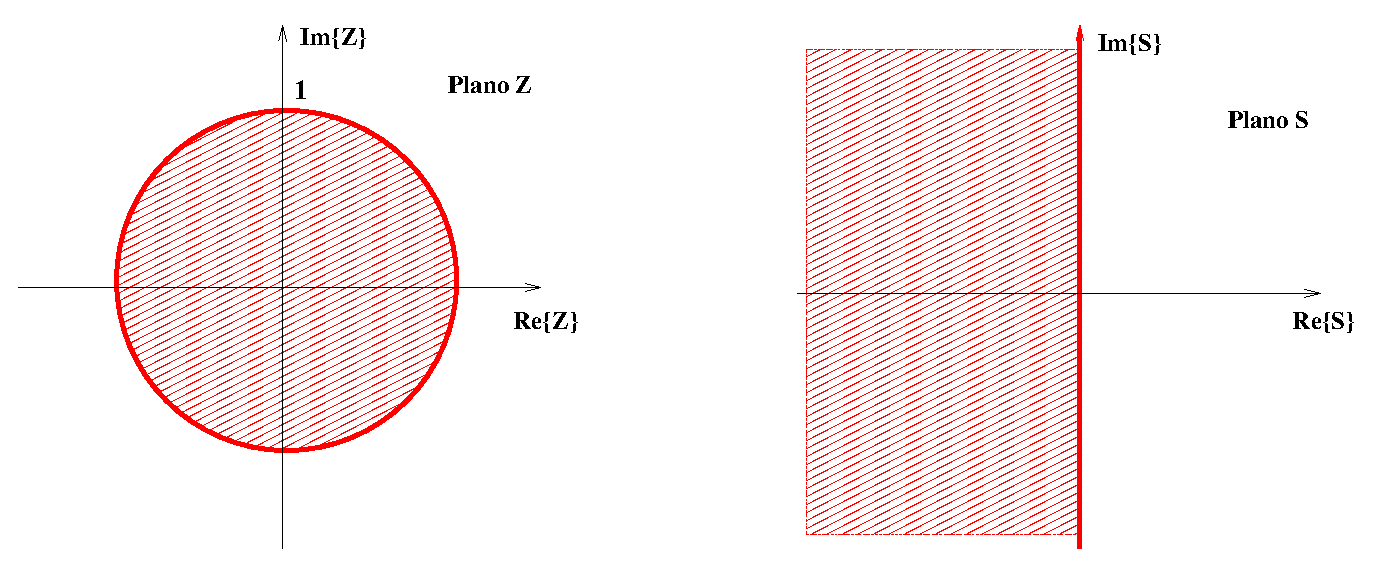
\includegraphics[width=0.99\textwidth]{figs/planosSZ.eps}
\end{figure}
\begin{equation*}
   \qquad z = re^{j\omega} \qquad\qquad\qquad\qquad s = \Sigma + j\Omega 
\end{equation*}
\end{slide}

\section[slide=true]{Região de convergência}
\begin{slide}{Convergência da Transformada Z}
Estabelecendo convergência
      \begin{align*}
         \left | \sum_{n=-\infty}^\infty x[n]z^{-n}\right| &= \left |\sum_{n=-\infty}^\infty x[n]r^{-n}e^{-j\omega n}\right |<\infty\\
         \left |\sum_{n=-\infty}^\infty x[n]r^{-n}e^{-j\omega n}\right |&\leq  \sum_{n=-\infty}^\infty |x[n]r^{-n}e^{-j\omega n}|\\
                                           &\leq  \sum_{n=-\infty}^\infty |x[n]r^{-n}| < \infty
      \end{align*}
\begin{itemize}
      \item Em relação à transformada de Fourier há um grau de liberdade adicional: variável $r$ 
\end{itemize}

\end{slide}

\begin{slide}{Região de convergência}
Definição
%\begin{itemize}
%   \item Região de convergência
   \begin{itemize}
      %\item Grau de liberdade adicional (variável $r$) 
      %\begin{itemize}
      %   \item Permite calcular a Transformada Z de sinais que não possuem Transformada de Fourier
      % \end{itemize}
      \item Pontos no plano Z, cujos valores de $r$ satisfazem à expressão 
      \begin{equation*}
           \sum_{n=-\infty}^\infty |x[n]r^{-n}| < \infty
      \end{equation*}
      \begin{figure}
      \centering
      \includegraphics[width=0.4\textwidth]{figs/planoZ}
   \end{figure}
   \end{itemize}
%\end{itemize}
\end{slide}

% \begin{slide}{Defini\c c\~ao e noções iniciais}
% \begin{itemize}
%    \item Região de convergência
%    \begin{itemize}
%       \item Pontos no plano Z, cujos $r$ atendem a 
%       \begin{equation*}
%            \sum_{n=-\infty}^\infty |x[n]r^{-n}| < \infty
%       \end{equation*}
%    \begin{figure*}[h]
%       \centering
%       \includegraphics[width=0.45\textwidth]{planoZ.eps}
%    \end{figure*}
%     \end{itemize}
% \end{itemize}
% \end{slide}
% 
\section[slide=true]{Polos e zeros}
\begin{slide}{Definições}
%\begin{itemize}
%   \item Polos e Zeros
   \begin{itemize}
      \item Polos: pontos ($p$) no plano Z para os quais \begin{equation*}\lim_{z\rightarrow p}X(z)= \infty \end{equation*}
      \item Zeros: pontos ($c$) no plano Z para os quais \begin{equation*} \lim_{z\rightarrow c}X(z) = 0 \end{equation*}
   \end{itemize}
%\end{itemize}
\end{slide}

\begin{slide}{Transformada Z na forma polinomial}
%\begin{itemize}
%   \item Polos e Zeros
   \begin{itemize}
      \item Para transformadas na forma de razão de polinômios:
      \begin{equation*}
           X(z) = \frac{P(z)}{Q(z)}
      \end{equation*}
      \begin{itemize}
         \item Polos: raízes de $Q(z)$
         \item Zeros: raízes de $P(z)$
      \end{itemize}
    \end{itemize}
%\end{itemize}
\end{slide}

\section[slide=true]{Exemplos}
\begin{slide}{Primeiros exemplos}
%\begin{itemize}
%   \item Exemplos
   \begin{itemize}
      \item Achar $X(z)$ e a região de convergência (ROC)
      \begin{enumerate}
         \item[a)] $x_1[n] = a^nu[n]$
         \item[b)] $x_2[n] = -a^nu[-n-1]$
         \item[c)] $x_3[n] = (1/2)^nu[n]+(-1/3)^nu[n]$
         \item[d)] $x_4[n] = -(1/2)^nu[-n-1]+(-1/3)^nu[n]$
         \item[e)] $x_5[n]=\begin{cases}a^n, & 0\leq n \leq N-1\\0, & \text{outro caso} \end{cases}$
      \end{enumerate}
    \end{itemize}
%\end{itemize}
\end{slide}

\begin{slide}{Resultados de (a) e (b)}
%\begin{itemize}
%   \item Exemplos (Continuação)
   \begin{itemize}
      \item $x_1[n] = a^nu[n]$
      \begin{equation*}
          X_1(z) = \frac{1}{1-az^{-1}} = \frac{z}{z-a}, \qquad |z|>|a|
      \end{equation*}
      \pause
      \item $x_2[n] = -a^nu[-n-1]$
      \begin{equation*}
          X_2(z) = \frac{1}{1-az^{-1}} = \frac{z}{z-a}, \qquad |z|<|a|
      \end{equation*}
   \end{itemize}
%\end{itemize}
\end{slide}

\begin{slide}{Comentários sobre (a) e (b)}
%\begin{itemize}
%   \item Exemplos (Continuação)
   \begin{align*}
          X_1(z) &= \frac{1}{1-az^{-1}} = \frac{z}{z-a}, \qquad |z|>|a|\\
          X_2(z) &= \frac{1}{1-az^{-1}} = \frac{z}{z-a}, \qquad |z|<|a|
      \end{align*}
    \begin{figure}
      \centering
      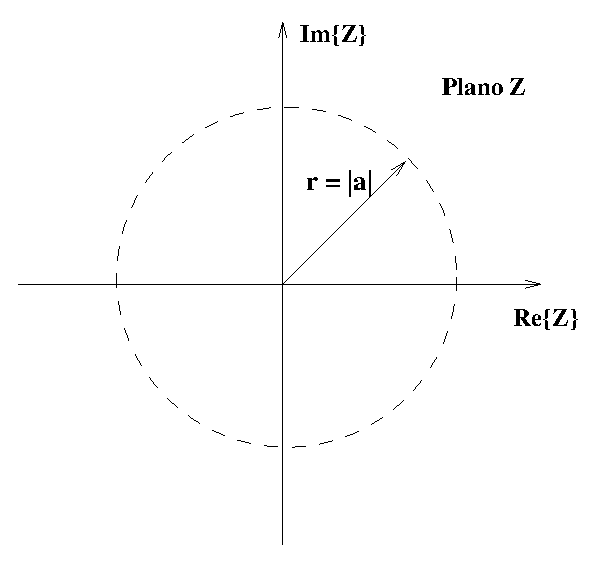
\includegraphics[width=0.45\textwidth]{figs/ex0102.eps}
   \end{figure}
%\end{itemize}
\end{slide}

 \begin{slide}{Resultados de (c) e (d)}
%\begin{itemize}
%   \item Exemplos (Continuação)
   \begin{itemize}
      \item $x_3[n] = (1/2)^nu[n]+(-1/3)^nu[n]$
      \begin{equation*}
          X_3(z) = \frac{2z\left ( z - \frac{1}{12} \right )}{\left ( z-\frac{1}{2}\right )\left ( z+\frac{1}{3}\right )}, \qquad |z| > \frac{1}{2}
      \end{equation*}
      \pause
      \item $x_4[n] = -(1/2)^nu[-n-1]+(-1/3)^nu[n]$
      \begin{equation*}
          X_4(z) = \frac{2z\left ( z - \frac{1}{12} \right )}{\left ( z-\frac{1}{2}\right )\left ( z+\frac{1}{3}\right )}, \qquad \frac{1}{3} < |z| < \frac{1}{2}
      \end{equation*}
   \end{itemize}
%\end{itemize}
\end{slide}

\begin{slide}{Resultado do item (e)}
%\begin{itemize}
%   \item Exemplos (Continuação)
   \begin{itemize}
      \item $x_5[n]=\begin{cases}a^n, & 0\leq n \leq N-1\\0, & \text{outro caso} \end{cases}$
      \begin{align*}
          X_5(z) &= \sum_{n=0}^{N-1}a^nz^{-n}\\
                 &= 1 + az^{-1} + a^2z^{-2} + \cdots a^{N-1}z^{-N+1}\\
                 &= \frac{z^N-a^N}{z^{N-1} ( z - a )}, \qquad z\neq 0
      \end{align*}
   \end{itemize}
%\end{itemize}
\end{slide}

\begin{note}{Equações complexas 01}
Considerando que $a\in  \mathbb{C}$ e $z \in  \mathbb{C}$: 
      \begin{align*}
         a &= |a|e^{j\theta}\\
         z &= re^{j\omega}
      \end{align*}
A solução da equação $z^N -a^N = 0$ segue os seguintes passos:
      \begin{align*}
          z^N -a^N &= 0\\
               z^N &= a^N\\
      \left [re^{j\omega}\right ]^N &=  \left [|a|e^{j\theta}\right ]^N\\
      \end{align*}
A igualdade deve ser verificada em \emph{módulo} e \emph{fase}
\end{note}

\begin{note}{Equações complexas 02}

% Continuando,
%       \begin{equation*}
%          \left [re^{j\omega}\right ]^N =  \left [|a|e^{j\theta}\right ]^N
%       \end{equation*}
%:
\begin{itemize}
   \item Magnitude
      \begin{align*}
          r^N &= |a|^N\\
          r   &= |a|
      \end{align*}
   \item Fase
      \begin{align*}
          e^{j\omega N} &= e^{j\theta N}\\
          %e^{j\omega N} &= e^{j\theta N}e^{jk2\pi}\\
          e^{j\omega N} &= e^{j(\theta N + k2\pi )}\\
          e^{j\omega N} &= e^{j(\theta N + k2\pi )}\\
          \omega  &= \theta + \frac{k2\pi}{N}, \qquad k = 0,1,\cdots ,N-1
      \end{align*}
   \end{itemize}
\end{note}

\begin{note}{Equações complexas 03}
%\begin{itemize}
%   \item Nota: Equações complexas
%       \begin{align*}
%            e^{j\omega N} &= e^{j(\theta N + k2\pi )}\\
%           \omega  &= \theta + \frac{k2\pi}{N}, \qquad k = 0,1,\cdots ,N-1
%       \end{align*}
      Logo, as raízes de $z^N-a^n =0$ são:
      \begin{equation*}
         z_k = |a|e^{j(\theta + \frac{k2\pi}{N})}, \qquad k = 0,1,\cdots ,N-1
      \end{equation*}
%   \end{itemize}
\end{note}

\begin{slide}{Polos e zeros para item (e)}
%\begin{itemize}
%   \item Exemplos (Continuação)
   \begin{equation*}
      X_5(z)=\frac{z^N-a^N}{z^{N-1}(z-a)},\qquad  |a| = 2, \theta = 0, N=8
   \end{equation*}
   \begin{figure}
      \centering
      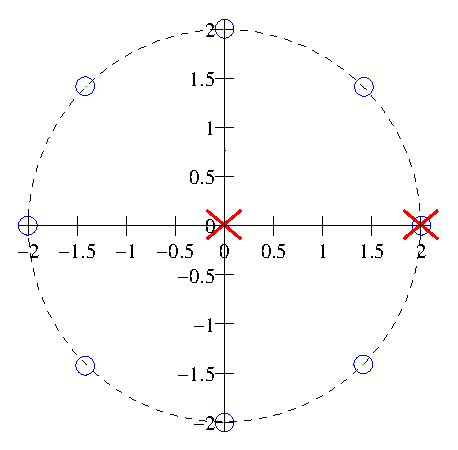
\includegraphics[width=0.45\textwidth]{figs/ex5.eps}
   \end{figure}
%\end{itemize}
\end{slide}

\section[slide=true]{Propriedades da RDC}
\begin{slide}{Propriedade 01}
\begin{itemize}
   \item P1: A RDC é um anel centrado na origem, tal que
   \begin{equation*}
      0\leq r_R < |z| < r_L \leq\infty
   \end{equation*}
   \begin{figure}
      \centering
      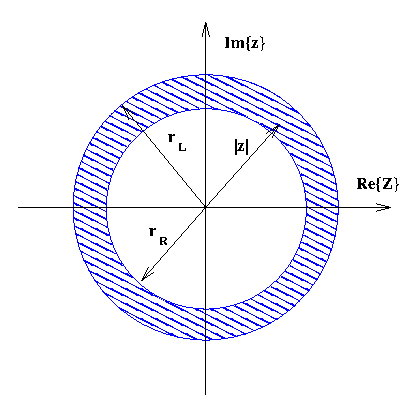
\includegraphics[width=0.45\textwidth]{figs/p1.eps}
   \end{figure}
\end{itemize}
\end{slide}

\begin{slide}{Propriedade 02}
\begin{itemize}
   \item P2: A \emph{transformada de Fourier} de $x[n]$ converge absolutamente se, e somente se, a RDC incluir a circunferência de raio unitário.
   \begin{figure}
      \centering
      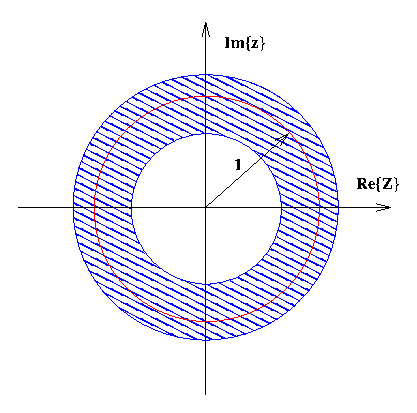
\includegraphics[width=0.45\textwidth]{figs/p2.eps}
   \end{figure}
\end{itemize}
\end{slide}

\begin{slide}{Propriedades 03 e 04}
\begin{itemize}
   \item P3: A RDC não pode conter nenhum polo.
   \item P4: Se $x[n]$ for uma \textcolor{red}{sequência de duração finita}, a RDC é todo o plano $Z$, exceto eventualmente os pontos $z=0$ e/ou $z=\infty$.
   \begin{itemize}
      \item Sequência de duração finita: os elementos de $x[n]$ são nulos, exceto em \begin{equation*} -\infty < N_1 \leq n \leq N_2 < \infty\end{equation*}
   \end{itemize} 
\end{itemize}
\end{slide}

\begin{slide}{Exemplo 01 da P4}
%\begin{itemize}
%   \item P4:
   \begin{itemize}
      \item 1º exemplo: $N_1=0$ \begin{equation*}X(z) = 1+x[1]z^{-1}+x[2]z^{-2}+ \cdots +x[N_2]z^{-N_2}\end{equation*}
   $X(z)$ converge para qualquer valor de $z$, menos $z=0$. Ou seja, $z =0$ é um polo.
   \end{itemize} 
%\end{itemize}
\end{slide}

\begin{slide}{Exemplo 02 da P4}
%\begin{itemize}
%   \item P4:
   \begin{itemize}
      \item 2º exemplo: $N_2=0$ \begin{equation*}X(z) = x[N_2]z^{-N_2}+ \cdots +x[-2]z^{2}+x[-1]z+1\end{equation*}
    $X(z)$ converge para qualquer valor de $z$, menos $z=\infty$:
   \begin{equation*}
      \lim_{z\rightarrow\infty}X(z) = \infty.
   \end{equation*} 
   
   Ou seja, $z=\infty$ é um polo.
   \end{itemize} 
%\end{itemize}
\end{slide}

\begin{slide}{Propriedade 05}
\begin{itemize}
   \item P5: Se $x[n]$ for uma \textcolor{red}{sequência ``à direita''} (\emph{right-sided}), a RDC se extende \textcolor{red}{para fora} a partir do polo finito mais externo.
   \begin{itemize}
      \item \textcolor{red}{Sequência ``à direita''}: $x[n]=0$ para $ n<N_1<\infty $
   \end{itemize}
   \begin{figure}
      \centering
      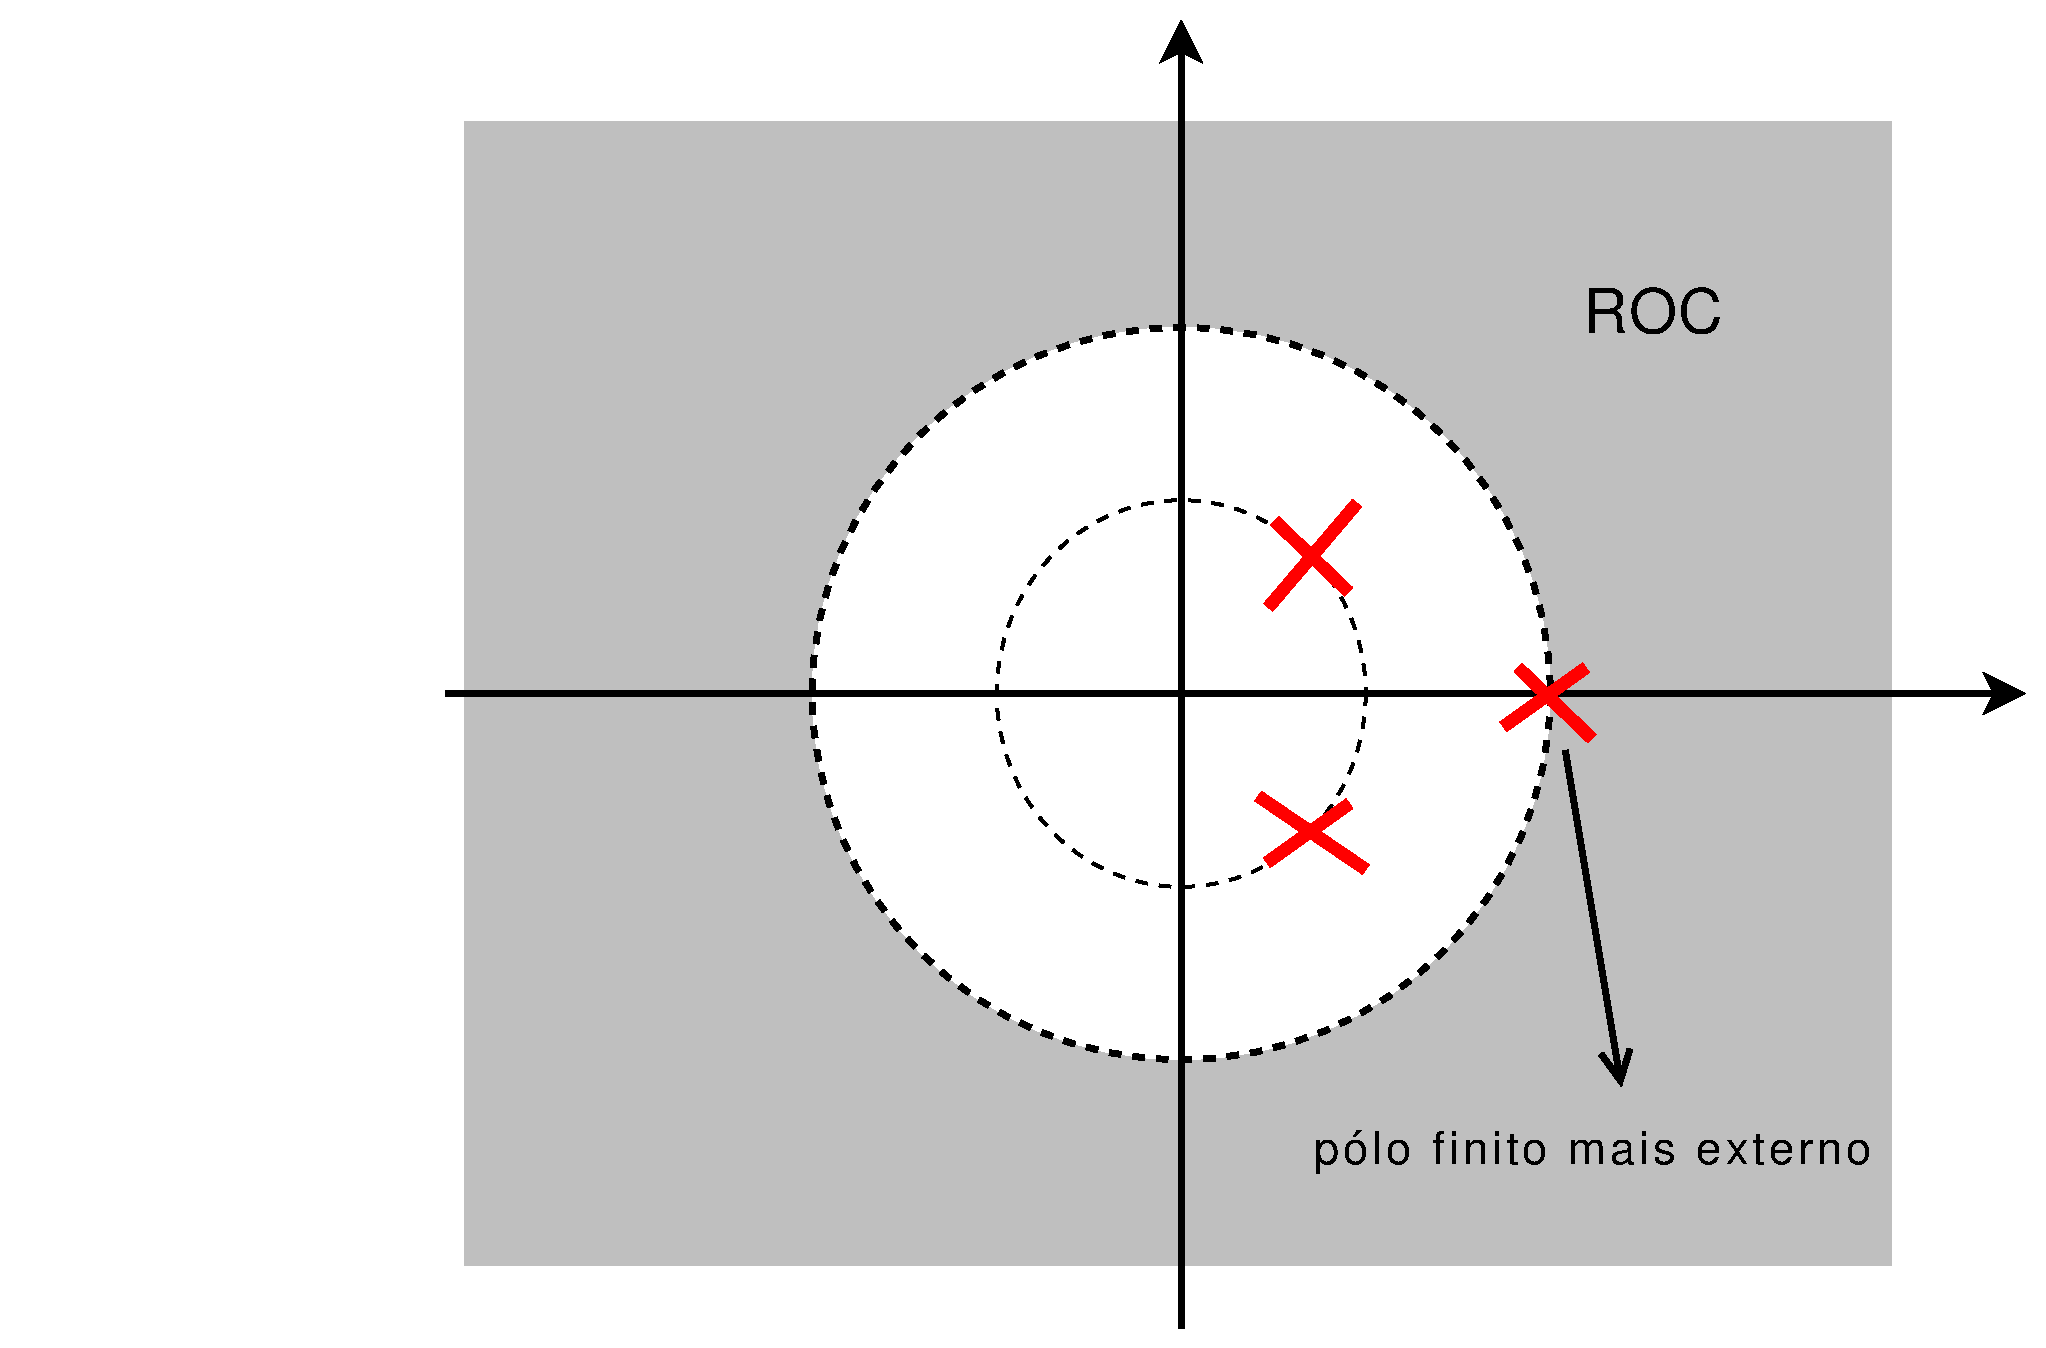
\includegraphics[width=0.55\textwidth]{figs/p5.eps}
   \end{figure}
\end{itemize}
\end{slide}

\begin{slide}{Propriedade 06}
\begin{itemize}
   \item P6: Se $x[n]$ for uma \textcolor{red}{sequência ``à esquerda''} (\emph{left-sided}), a RDC se extende \textcolor{red}{para dentro} a partir do polo finito mais interno.
   \begin{itemize}
      \item \textcolor{red}{Sequência ``à esquerda''}: $x[n]=0$ para $n>N_2>-\infty $
   \end{itemize}
   \begin{figure}
      \centering
      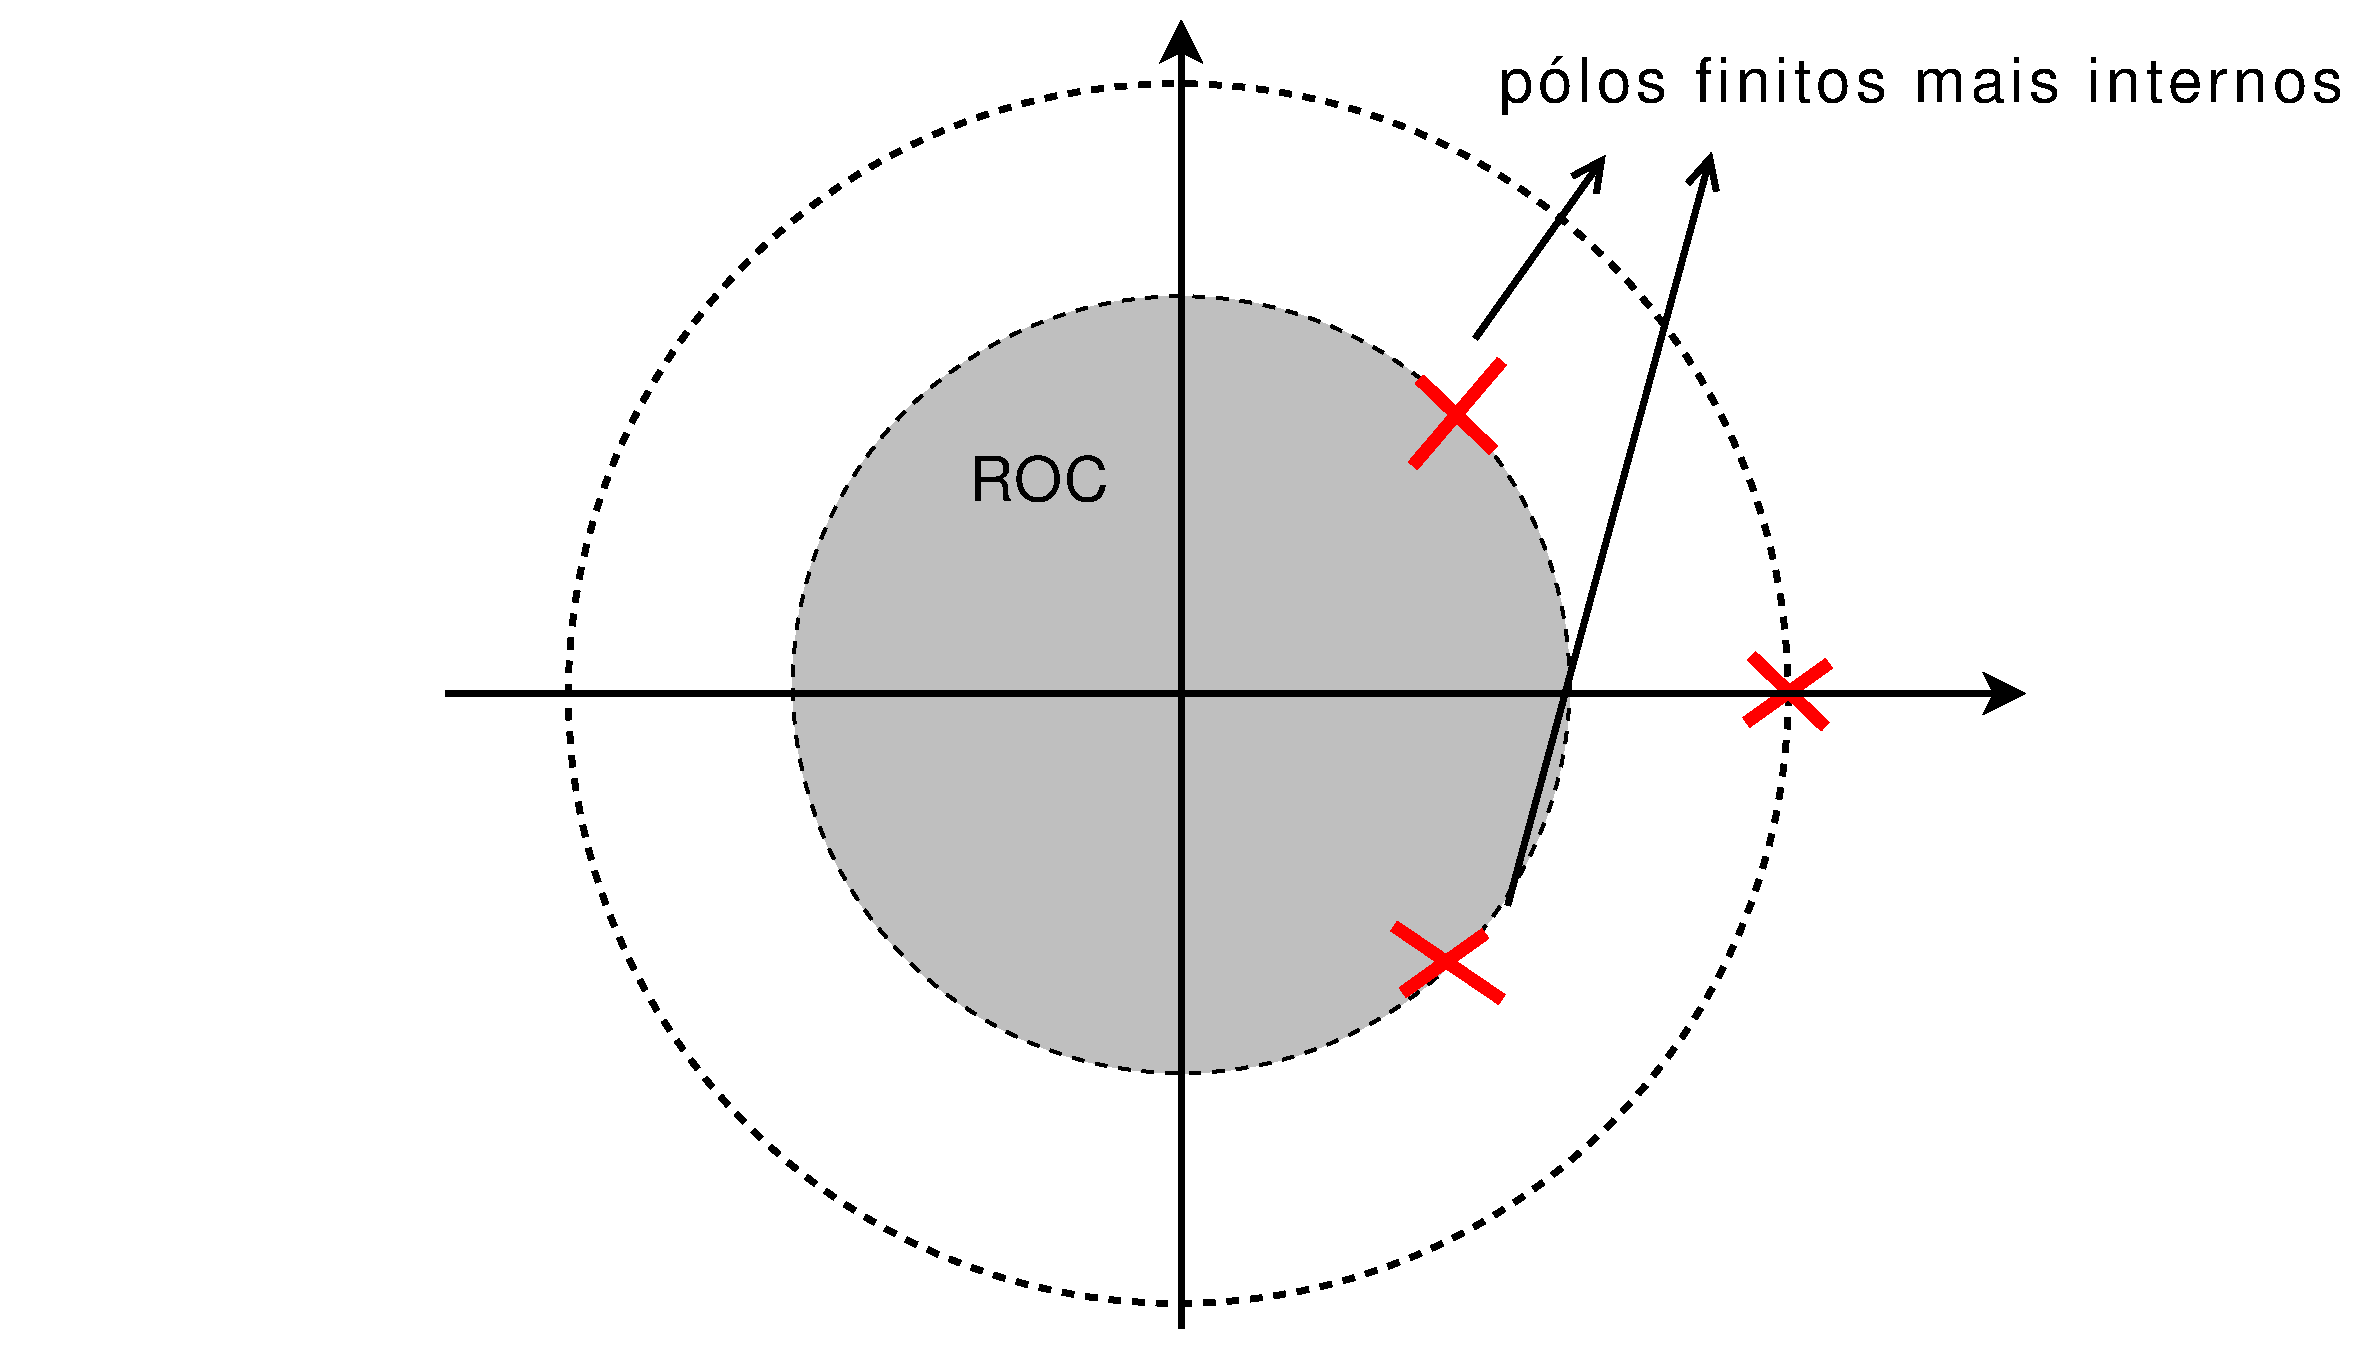
\includegraphics[width=0.55\textwidth]{figs/p6.eps}
   \end{figure}
\end{itemize}
\end{slide}

\begin{slide}{Propriedade 07}
\begin{itemize}
   \item P7: Se $x[n]$ for uma \textcolor{red}{sequência ``à esquerda e à direita''} (\emph{two-sided}), a RDC é um anel no plano $Z$ limitado por polos.
   \begin{figure}
      \centering
      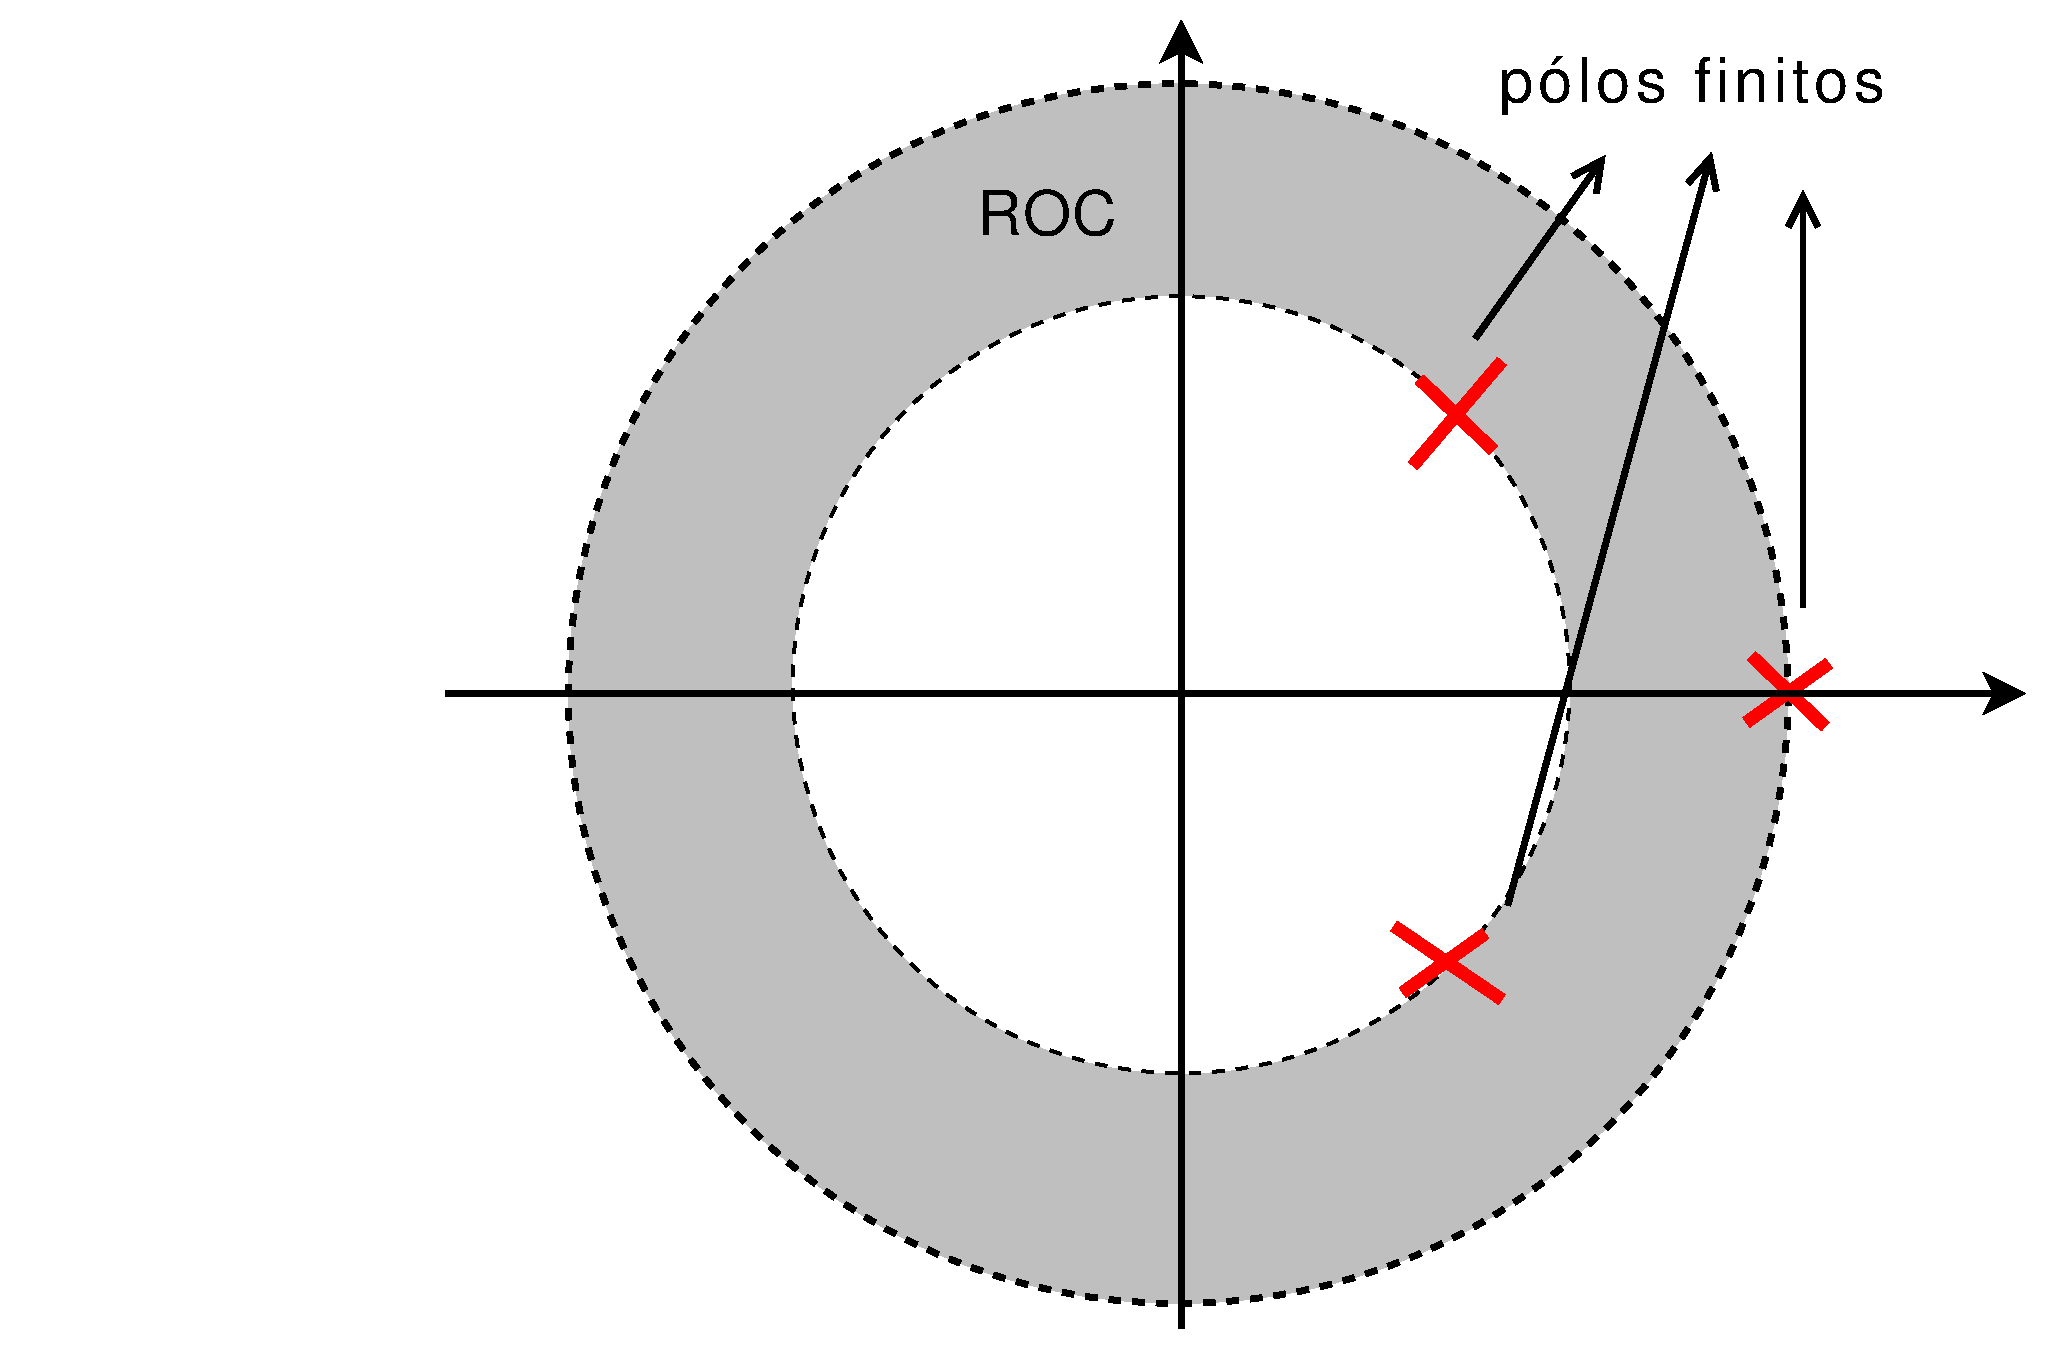
\includegraphics[width=0.55\textwidth]{figs/p7.eps}
   \end{figure}
\end{itemize}
\end{slide}

\begin{slide}{Propriedades da RDC}
\begin{itemize}
   \item Diferentes RDCs para o mesmo conjunto de polos
   \begin{figure}
      \centering
      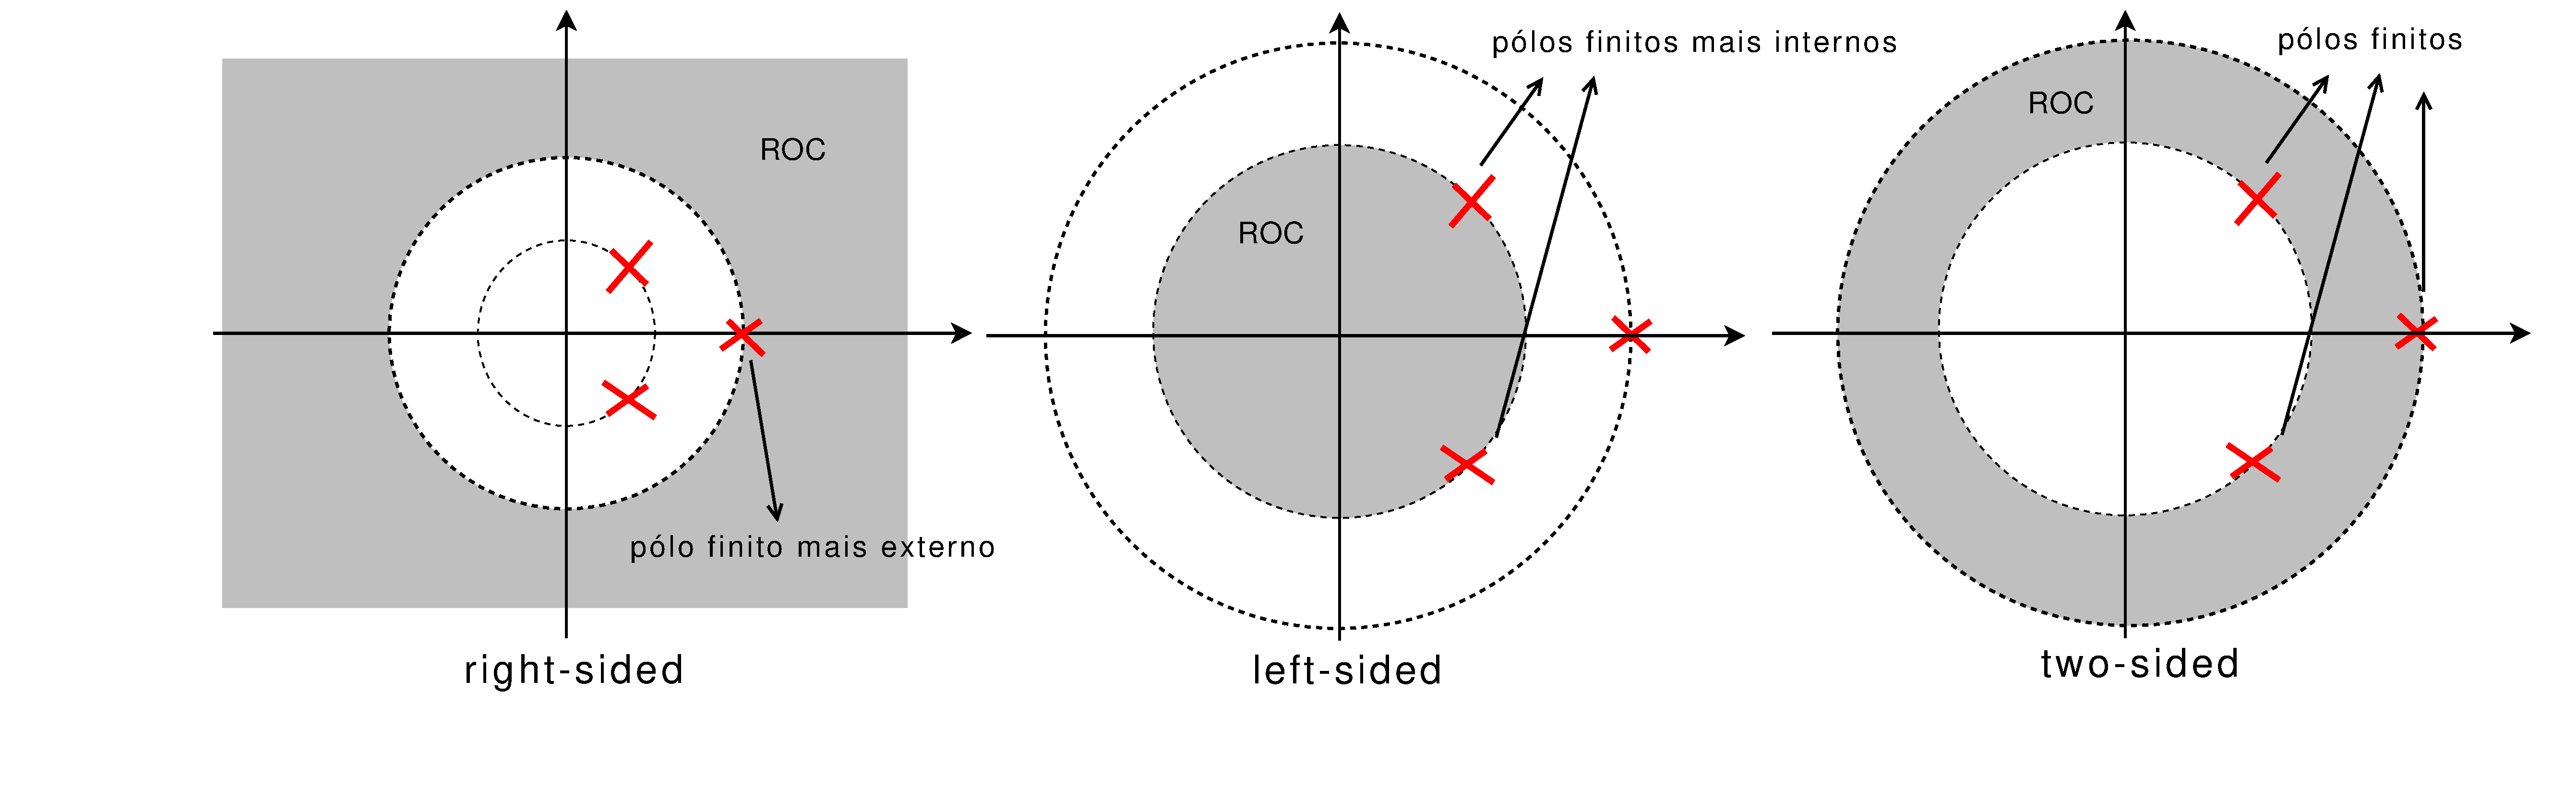
\includegraphics[width=\textwidth]{figs/p_roc.eps}
   \end{figure}
   estão associadas a diferentes sequências $x[n]$.
\end{itemize}
\end{slide}


\begin{slide}{Exercícios}
\begin{itemize}
  \item Calcular a transformada Z e a RDC
  \begin{enumerate}
     \item [a)]$\delta[n]$
     \item [b)]$u[n]$
     %\item [c)]$na^nu[n]$
     %\item [d)]$-na^nu[-n-1]$
     \item [c)]$\text{cos}(\omega_kn)u[n]$
     \item [d)]$\text{sen}(\omega_kn)u[n]$
     \item [e)]$r^n\text{sen}(\omega_kn)u[n]$
  \end{enumerate}
\end{itemize}
\end{slide}

\section[slide=true]{Transformada Z inversa}
\begin{slide}{Método da inspeção}
\begin{itemize}
   \item ``Reconhecer pares de transformada''\\
        \begin{equation*}X(z) = \frac{1}{1-0,5z^{-1}}, \qquad |z|>0,5 \end{equation*}
        \begin{equation*}X(z) = \frac{1}{1+(2e^{j5})z^{-1}}, \qquad |z|>2 \end{equation*}
        \begin{equation*}X(z) = \frac{10}{1+(2e^{j5})z^{-1}}, \qquad |z|<2 \end{equation*}
        \begin{equation*}X(z) = \frac{z^{-k}}{1+(2e^{j5})z^{-1}}, \qquad |z|>2 \end{equation*}
\end{itemize}
\end{slide}

\begin{slide}{Expansão em frações parciais}
\begin{itemize}
   \item Transformada Z na forma razão de polinômios
   \begin{align*}
      X(z) &= \frac{\sum_{k=0}^M b_k z^{-k}}{\sum_{k=0}^N a_k z^{-k}}\\
           &= \frac{b_0}{a_0}\frac{\prod_{k=1}^M (1-c_k z^{-1})}{\prod^N_{k=1}(1-d_k z^{-1})}
           %&= \frac{z^{N}\sum_{k=0}^M b_k z^{M-k}}{z^{M}\sum_{k=0}^N a_k z^{N-k}}
   \end{align*}
   \begin{itemize}
       \item Polos distintos de 1ª ordem e $M<N$
      \begin{align*}
         X(z) &= \sum_{k=1}^N\frac{A_k}{1-d_kz^{-1}}\\
         A_k &= X(z)\left .(1-d_kz^{-1})\right |_{z=d_k}
      \end{align*}
   \end{itemize}
\end{itemize}
\end{slide}

\begin{slide}{Exemplo 01}
\begin{itemize}
   \item Calcule a transformada Z inversa de
      \begin{equation*}
         X(z) = \frac{1}{\left (1-\frac{1}{4}z^{-1} \right ) \left (1-\frac{1}{2}z^{-1} \right )}, \qquad |z|>1/2
      \end{equation*}\pause
      
      \begin{equation*}
         x[n] = -\left (\frac{1}{4}\right )^n u[n] + 2\left ( \frac{1}{2} \right )^n u[n]
      \end{equation*}
\end{itemize}
\end{slide}


\begin{slide}{Expansão em frações parciais 2}
\begin{itemize}
   \item Polos distintos de 1ª ordem e $M\geq N$
   \begin{equation*}
      X(z) = \sum_{r=0}^{M-N}B_rz^{-r}+\sum_{k=1}^N\frac{A_k}{1-d_kz^{-1}}
   \end{equation*}
   Divisão polinomial até o resto ser de menor ordem que o denominador.
\end{itemize}
\end{slide}


\begin{slide}{Exemplo 02}
\begin{itemize}
   \item Calcule a transformada Z inversa de
      \begin{equation*}
          X(z) = \frac{1+2z^{-1}+z^{-2}}{1-\frac{3}{2}z^{-1}+\frac{1}{2}z^{-2}}, \qquad |z|>1
      \end{equation*}\pause
      
      \begin{equation*}
          x[n] = 2\delta [n]-9\left (\frac{1}{2} \right )^nu[n]+8u[n]
      \end{equation*}
\end{itemize}
\end{slide}

\begin{slide}{Expansão em frações parciais 3}
\begin{itemize}
   \item Polos múltiplos e $M\geq N$\footnotesize{
   \begin{equation*}
      X(z) = \sum_{r=0}^{M-N}B_rz^{-r}+\sum_{k=1, k\neq i}^N\frac{A_k}{1-d_kz^{-1}}+
      \sum_{m=1}^s\frac{C_m}{\left ( 1-d_iz^{-1} \right ) ^m}
   \end{equation*}}
   onde $X(z)$ tem um polo de ordem $s$ em $z = d_i$ e 
   \begin{equation*}
      C_m = \frac{1}{\left ( s - m\right )!\left ( -d_i\right )^{s-m}}\left \{ \frac{d^{s-m}}{dw^{s-m}} \left [ \left ( 1-d_iw \right )^s X\left ( w^{-1}\right )\right ]\right \}_{w = d_i^{-1}}
   \end{equation*}

\end{itemize}
\end{slide}


\begin{slide}{Expansão em série de potência}
\begin{itemize}
   \item Identificação dos coeficientes multiplicativos dos termos $z^n$
   \begin{align*}
      X(z) &= \sum_{n=-\infty}^{\infty}x[n]z^{-n}\\
           &= \cdots + x[-1]z+x[0]+x[1]z^{-1}+ \cdots
   \end{align*}
\end{itemize}
\end{slide}


\begin{slide}{Exemplo 03}
\begin{itemize}
   \item Calcule a transformada Z inversa da sequência de comprimento finito
      \begin{equation*}
         X(z) = z^2(1-0,5z^{-1})(1+z^{-1})(1-z^{-1})
      \end{equation*}\pause
     \begin{equation*}
         x[n]= \delta [n+2] - 1/2\delta [n+1] - \delta [n] +1/2 \delta [n-1]
      \end{equation*}
\end{itemize}
\end{slide}

\begin{slide}{Exemplo 04}
\begin{itemize}
   \item Calcule a transformada Z inversa de
   \begin{equation*}
       X(z) = \log (1-az^{-1}), \qquad |z|>a
   \end{equation*}
    
   \begin{align*}
         & \log(1+x), \qquad |x|<1\\ %}
        X(z) &= \sum_{n=1}^\infty\frac{(-1)^{n+1}a^n}{n}z^{-n}\\%}\\
        x[n] &= \begin{cases}\frac{(-1)^{n+1}a^n}{n}, & n\geq 1\\ 0, & n<1 \end{cases}%}
      \end{align*}
   
\end{itemize}
\end{slide}

\begin{slide}{Teorema dos resíduos}
\begin{itemize}
   \item Seja $X(z)$ uma função complexa analítica no interior de um contorno fechado $C$, incluindo o próprio contorno, exceto em um número finito de pontos singulares $p_n$ no interior de $C$. Neste caso, a equação seguinte se aplica.
   \begin{equation*}
      \oint_{C}{X(z)dz} = 2\pi j \sum_{k = 1}^{K}\operatorname*{res}_{z = p_k}\left \{ X(z)\right \}
   \end{equation*}
   com a integral avaliada no sentido anti-horário de $C$.
\end{itemize}
\end{slide}

\begin{slide}{Determinação dos resíduos}
\begin{itemize}
   \item Resíduos
   \begin{equation*}
      \operatorname*{res}_{z = p_k} \left \{ X(z)\right \}= \frac{1}{\left ( m - 1 \right )! }\left \{ \frac{d^{m-1}}{dz^{m-1}} \left [ \left ( z-p_k \right )^m X\left ( z\right )\right ]\right \}_{z = p_k}
   \end{equation*}
   \item Transformada Z inversa
   \begin{equation*}
      x[n] = \frac{1}{2\pi j}\oint_{C}{X(z)z^{n-1}dz} = \sum_{k = 1}^{K}\operatorname*{res}_{z = p_k}\left \{ X(z)z^{n-1}\right \}
   \end{equation*}
\end{itemize}
\end{slide}

\begin{slide}{Exemplo 05}
Determine a transformada Z inversa de
   \begin{equation*}
      X(z) = \frac{z^2}{(z-0,2)(z+0,8)}
   \end{equation*}
   dado 	que $x[n]$ é uma sequência à direita.\pause
   \begin{equation*}
      x[n] = [(0,2)^{n+1} -(-0,8)^{n+1}] u[n+1]
   \end{equation*}
\end{slide}


\section[slide=true]{Propriedades da Transformada Z}
\begin{slide}{Propriedades}
\begin{itemize}
 \item Deduzir as propriedades da Transformada Z
   \begin{itemize}
      \item Linearidade 
      \begin{equation*} 
        \alpha x[n] + \beta y[n] \overset{Z}{\longleftrightarrow} \alpha X(z)+\beta Y(z), \quad \text{RDC contém } R_x\cap R_y
      \end{equation*}
      
      \item Deslocamento em $n$
      \begin{equation*} 
        x[n-n_0]  \overset{Z}{\longleftrightarrow} z^{-n_0}X(z), \quad \text{RDC}= R_x \text{ (atenção em } z= 0 \text{ e } z= \infty \text{)}
      \end{equation*}
      
      \item Mutiplicação por uma sequência exponencial
      \begin{equation*} 
        z_0^nx[n] \overset{Z}{\longleftrightarrow} X(z/z_0), \quad \text{RDC}=|z_0| R_x
      \end{equation*}
      
      \item Diferenciação de $X(z)$
      \begin{equation*} 
        nx[n] \overset{Z}{\longleftrightarrow} -z\frac{X(z)}{dz}, \quad \text{RDC}=R_x
      \end{equation*}
      
%      \item Conjugação de uma sequência complexa
%      \item Reversão de $n$
%      \item Convolução de sequências
%      \item Teorema do valor inicial
   \end{itemize}
\end{itemize}
\end{slide}

\begin{slide}{Propriedades}
\begin{itemize}
 \item Deduzir as propriedades da Transformada Z
   \begin{itemize}
      \item Conjugação de uma sequência complexa
      \begin{equation*} 
        x^*[n] \overset{Z}{\longleftrightarrow} X^*(z^*), \quad \text{RDC}=R_x
      \end{equation*}
      \item Reversão de $n$
      \begin{equation*} 
        x^*[-n] \overset{Z}{\longleftrightarrow} X^*(1/z^*), \quad \text{RDC}=\frac{1}{R_x}
      \end{equation*}
      \item Convolução de sequências
      \begin{equation*} 
        x[n]*y[n] \overset{Z}{\longleftrightarrow} X(z)Y(z), \quad \text{RDC contém } R_x\cap R_y
      \end{equation*}
      %\item Teorema do valor inicial
   \end{itemize}
\end{itemize}
\end{slide}

\end{document}
